%
% Main document
% ===========================================================================
% This is part of the document "Project documentation template".
% Authors: brd3, kaa1
%

%---------------------------------------------------------------------------
\documentclass{bfh_template}
\usepackage{tikz}
\usetikzlibrary{arrows,shadows}
\usepackage{pgf-umlsd}

%---------------------------------------------------------------------------
%  Read title, version number and date of the paper from the file:
%  title_version_def.tex
\providecommand{\titel}{Metropolitan-Sensor/Aktor-Netze unter Einsatz von LoRa und anderen Techniken}					%  Hier den Titel des Berichts/Thesis eingeben
\providecommand{\versionnumber}{1.0}			%  Hier die aktuelle Versionsnummer eingeben
\providecommand{\versiondate}{25.06.2016}		%  Hier das Datum der aktuellen Version eingeben


%---------------------------------------------------------------------------
\begin{document}                        % Start Document


%---------------------------------------------------------------------------
% Title Page and Abstract
%---------------------------------------------------------------------------
%\include{lead/titelseite_ohne_bild}	% activate for Titelseite ohne Bild
%
% Project documentation template
% ===========================================================================
% This is part of the document "Project documentation template".
% Authors: brd3, kaa1
%

\begin{titlepage}


% BFH-Logo absolute placed at (28,12) on A4 and picture (16:9 or 15cm x 8.5cm)
% Actually not a realy satisfactory solution but working.
%---------------------------------------------------------------------------
\setlength{\unitlength}{1mm}
\begin{textblock}{20}[0,0](28,12)
	
\includegraphics[scale=1.0]{pictures/BFH_Logo_B.png}
\end{textblock}

\begin{textblock}{154}(28,48)
	\begin{picture}(150,2)
		\put(0,0){\color{bfhgrey}\rule{150mm}{2mm}}
	\end{picture}
\end{textblock}

\begin{textblock}{154}[0,0](28,50)
	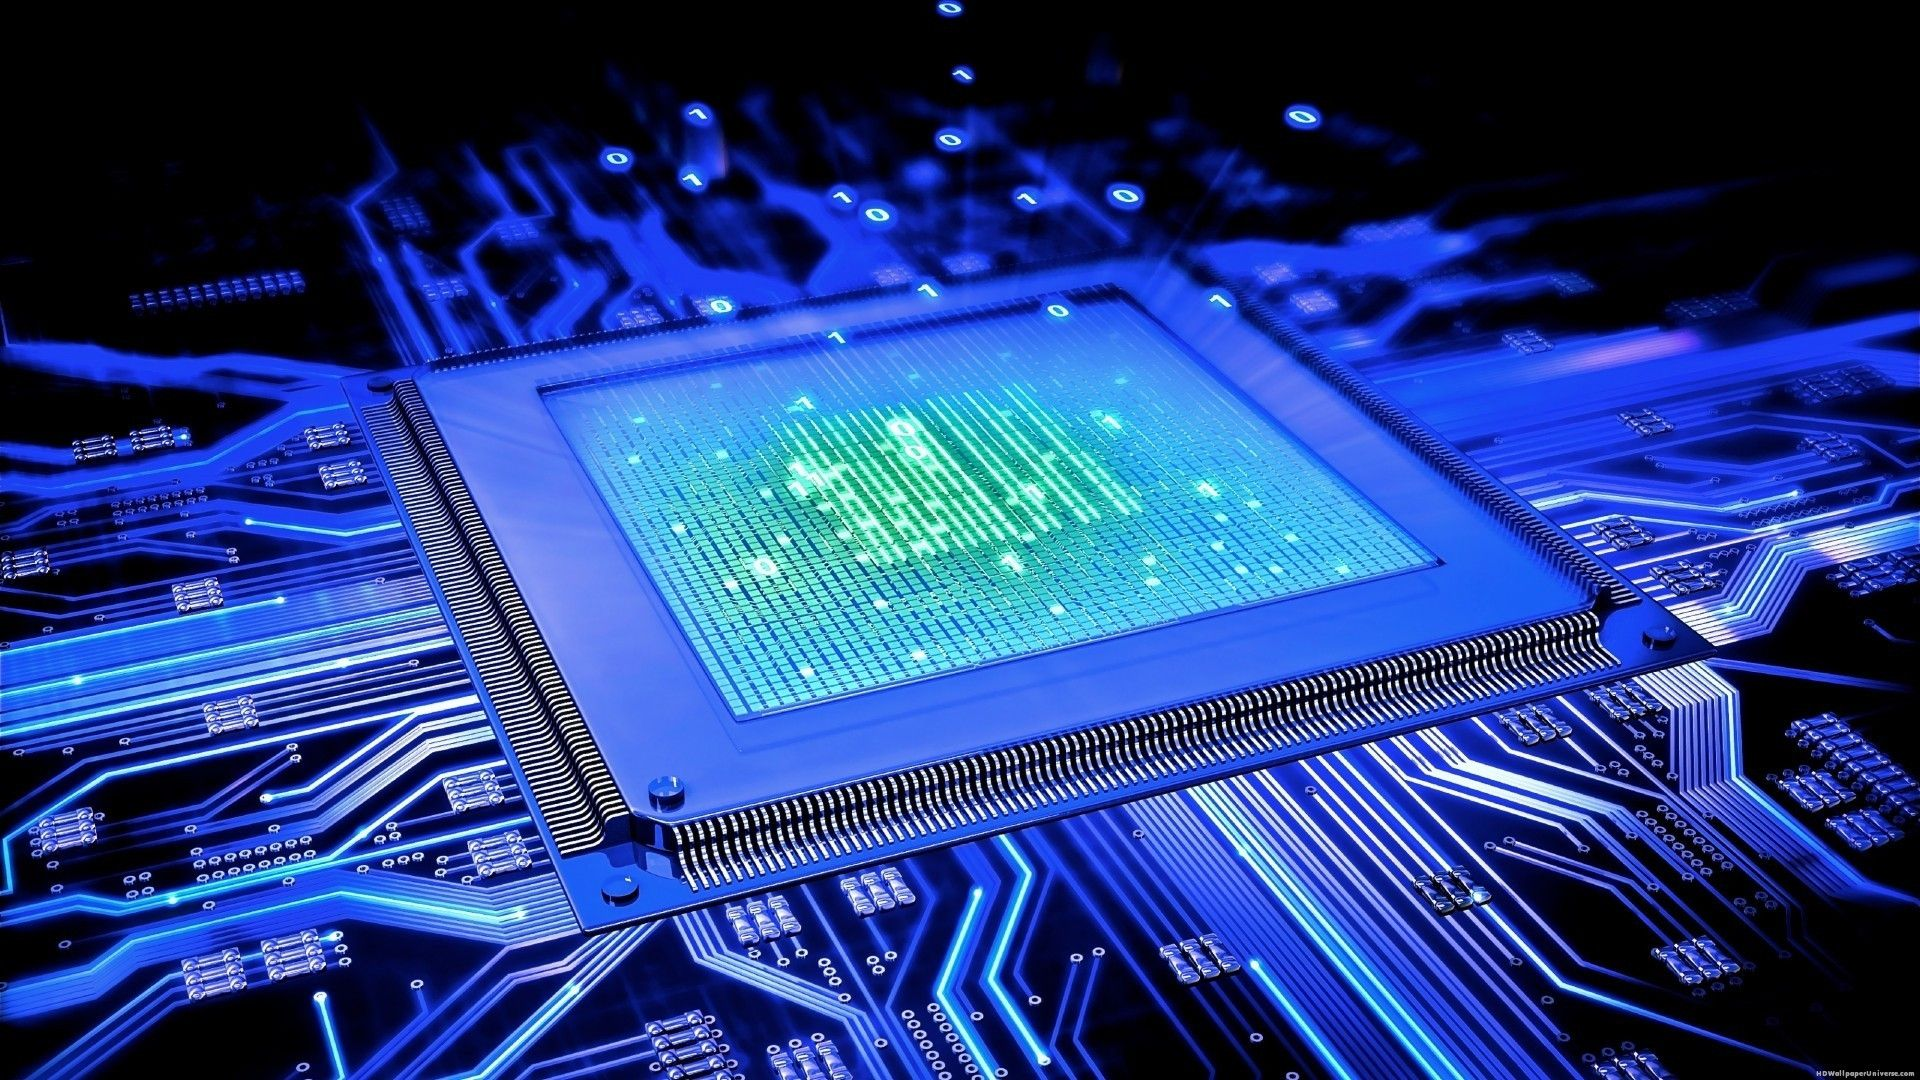
\includegraphics[height=85mm,width=150mm]{pictures/cs.jpg}
%\includegraphics[width=150mm]{pictures/network-782707_1280.png}			% Titelbild definieren
%1.764705882
\end{textblock}

\begin{textblock}{154}(28,135)
	\begin{picture}(150,2)
		\put(0,0){\color{bfhgrey}\rule{150mm}{2mm}}
	\end{picture}
\end{textblock}
\color{black}

% Institution / Titel / Untertitel / Autoren / Experten:
%---------------------------------------------------------------------------
\begin{flushleft}

\vspace*{115mm}

\fontsize{26pt}{28pt}\selectfont
\titel 								\\ % Titel aus der Datei lead/titel.tex lesen
\vspace{2mm}

% \fontsize{16pt}{20pt}\selectfont\vspace{0.3em}
% Subtitle 	\\ % Untertitel eingeben
% \vspace{5mm}

\fontsize{10pt}{12pt}\selectfont
\textbf{Projekt 2} \\ % eingeben
\vspace{3mm}

% Abstract (eingeben):
%---------------------------------------------------------------------------
%\begin{textblock}{150}(28,190)
%\fontsize{10pt}{12pt}\selectfont
%[Kurztext (Abstract) einfügen, falls gewünscht] \\
%Dieses Dokument dient als Vorlage für die Erstellung von Berichten nach den Richtlinien der BFH. Die Vorlage ist %in \LaTeX{} erstellt und unterstützt das automatische Erstellen von diversen Verzeichnissen, Literaturangaben, %Indexierung und Glossaren. Dieser kleine Text ist eine Zusammenfassung über das vorliegenden Dokument mit einer %Länge von 4 bis max. 8 Zeilen. \\
%Das Titelbild kann in den Zeilen 157/158 der Datei template.tex ein- oder ausgeschaltet werden.
%\end{textblock}

\begin{textblock}{150}(28,225)
\fontsize{10pt}{17pt}\selectfont
\begin{tabbing}
xxxxxxxxxxxxxxx\=xxxxxxxxxxxxxxxxxxxxxxxxxxxxxxxxxxxxxxxxxxxxxxx \kill
\\
\\
Studiengang:	\> Bachelor of Science Informatik	\\	% Namen eingeben
Autor:			\> Simon Wittwer, Marc Zimmermann	\\	% Namen eingeben
Betreuer:		\> Dr.~Andreas Danuser				\\	% Namen eingeben
% Experte:		\> Don Mutex						\\	% Namen eingeben
Datum:			\> \versiondate						\\	% aus Datei lead/versions.tex lesen
\end{tabbing}

\end{textblock}
\end{flushleft}

\begin{textblock}{150}(28,280)
\noindent
\color{bfhgrey}\fontsize{9pt}{10pt}\selectfont
Berner Fachhochschule | Haute école spécialisée bernoise | Bern University of Applied Sciences
\color{black}\selectfont
\end{textblock}


\end{titlepage}

%
% ===========================================================================
% EOF
%
				% activate for Titelseite mit Bild
% Versionenkontrolle :
% -----------------------------------------------

\null
\vfill

\begin{Large}
Versionen
\end{Large}

\fontsize{10pt}{18pt}\selectfont
\begin{tabbing}
xxxxxxxxxxx\=xxxxxxxxxxxxxxx\=xxxxxxxxxxxxxx\=xxxxxxxxxxxxxxxxxxxxxxxxxxxxxxxxxxxxxxxxxxxxxxx \kill
Version	\> Datum	\> Status		\> Bemerkungen		\\
0.1	\> 22.04.2016	\> Entwurf		\> Latex-Dokument eingerichtet	\\
0.1.1\> 23.04.2016	\> Entwurf		\> Kapitelstruktur erstellt \\
0.2	\> 12.06.2016	\> Entwurf		\> Anforderungen \\
0.3	\> 11.06.2016	\> Entwurf		\> Kapitel Einleitung \\
0.4	\> 18.06.2016	\> Entwurf		\> Kapitel Anwendungsfälle und Anforderungen \\
0.5	\> 20.06.2016	\> Entwurf		\> Kapitel Rahmenbedingungen \\
0.6	\> 20.06.2016	\> Entwurf		\> Kapitel Use Case Tresh \\
0.7	\> 23.06.2016	\> Entwurf		\> Kapitel Drahtlose Datenübertragung \\
0.8	\> 24.06.2016	\> Entwurf		\> Kapitel Prototyp, Resultate, Anhang \\
0.9	\> 25.06.2016	\> Entwurf		\> Management Summary, Fazit und Korrektur lesen \\
1.0	\> 25.06.2016	\> Final		\> Finale Version \\
\end{tabbing}


\cleardoubleemptypage
%\setcounter{page}{1}

\cleardoublepage
\phantomsection
% % \chapter*{Summary}\label{summary}
% \addcontentsline{toc}{chapter}{Summary}

\begin{abstract}
{\huge Management Summary\par} % parens are here to define the scope of \huge and \par
% \lipsum[1]
Diese Arbeit befasst sich im Rahmen des Projekt 2 mit verschiedenen Aspekten von \gls{iot}. Einerseits wird versucht mit der Auseinandersetzung von möglichen Use-Cases über verschiedene Branchen hinweg, ein Gefühl für das Marktpotential und die Herausforderungen von \gls{iot} zu entwickeln und daraus gleichzeitig wichtige Anforderungen an \gls{iotk} abzuleiten. Andererseits wird mit der Gegebüberstellung der wichtigsten Funktechnologien und deren Vor- und Nachteilen eine Übersicht verschafft und die auf Spreizbandmodulation basierende Technologie \gls{lora} vertieft betrachtet.\\
Um die verschiedenen Aspekte schliesslich zu kombinieren, wird der konkrete Use-Case \glqq{}Tresh\grqq{} vorgestellt und dessen Implementation und die gewonnenen Erfahrungen anhand eines Prototypen aufgezeigt.
\end{abstract}

% \chapter*{Summary}\label{summary}
% \addcontentsline{toc}{chapter}{Summary}

\begin{abstract}
{\huge Management Summary\par} % parens are here to define the scope of \huge and \par
% \lipsum[1]
Diese Arbeit befasst sich im Rahmen des Projekt 2 mit verschiedenen Aspekten von \gls{iot}. Einerseits wird versucht mit der Auseinandersetzung von möglichen Use-Cases über verschiedene Branchen hinweg, ein Gefühl für das Marktpotential und die Herausforderungen von \gls{iot} zu entwickeln und daraus gleichzeitig wichtige Anforderungen an \gls{iotk} abzuleiten. Andererseits wird mit der Gegebüberstellung der wichtigsten Funktechnologien und deren Vor- und Nachteilen eine Übersicht verschafft und die auf Spreizbandmodulation basierende Technologie \gls{lora} vertieft betrachtet.\\
Um die verschiedenen Aspekte schliesslich zu kombinieren, wird der konkrete Use-Case \glqq{}Tresh\grqq{} vorgestellt und dessen Implementation und die gewonnenen Erfahrungen anhand eines Prototypen aufgezeigt.
\end{abstract}

\cleardoubleemptypage

%---------------------------------------------------------------------------
% Table of contents
%---------------------------------------------------------------------------
\tableofcontents

%---------------------------------------------------------------------------
% Main part
%---------------------------------------------------------------------------
\cleardoublepage
\pagenumbering{arabic}
\include{chapters/demo.md}

%---------------------------------------------------------------------------
% Statement
%---------------------------------------------------------------------------
\cleardoublepage
\phantomsection
\addcontentsline{toc}{chapter}{Selbständigkeitserklärung}
\chapter*{Selbstständigkeitserklärung}
\label{chap:selbstaendigkeitserklaerung}

\vspace*{10mm}
Wir bestätigen mit unseren Unterschriften, dass wir unsere vorliegende Bachelorthesis selbstständig durchgeführt haben. Alle Informationsquellen (Fachliteratur, Besprechungen mit Fachleuten, usw.) und anderen Hilfsmittel, die wesentlich zu unserer Arbeit beigetragen haben, sind in unserem Arbeitsbericht im
Anhang vollständig aufgeführt. Sämtliche Inhalte, die nicht von uns stammen, sind mit dem genauen Hinweis auf ihre Quelle gekennzeichnet.

\vspace{15mm}

\begin{tabbing}
xxxxxxxxxxxxxxxxxxxxxxxxx\=xxxxxxxxxxxxxxxxxxxxxxxxxxxxxx\=xxxxxxxxxxxxxxxxxxxxxxxxxxxxxx\kill
Ort, Datum:		\> Bern, \versiondate \\ \\
Namen:	\> Simon Wittwer 	\> Marc Zimmermann \\ \\ \\ \\
Unterschriften:	\> ......................................\> ...................................... \\
\end{tabbing}


%---------------------------------------------------------------------------
% Glossary
%---------------------------------------------------------------------------
\cleardoublepage
\phantomsection
\addcontentsline{toc}{chapter}{Glossar}
% \renewcommand{\glossaryname}{Glossar}
\printglossary

%---------------------------------------------------------------------------
% Bibliography
%---------------------------------------------------------------------------
\cleardoublepage
\phantomsection
\nocite{*}
\addcontentsline{toc}{chapter}{Literaturverzeichnis}
\bibliographystyle{IEEEtranS}
\bibliography{references/bibliography}{}

%---------------------------------------------------------------------------
% Listings
%---------------------------------------------------------------------------
\cleardoublepage
\phantomsection
\addcontentsline{toc}{chapter}{Abbildungsverzeichnis}
\listoffigures

\cleardoublepage
\phantomsection
\addcontentsline{toc}{chapter}{Tabellenverzeichnis}
\listoftables

%---------------------------------------------------------------------------
% Index
%---------------------------------------------------------------------------
%\cleardoublepage
%\phantomsection
%\addcontentsline{toc}{chapter}{Stichwortverzeichnis}
%\renewcommand{\indexname}{Stichwortverzeichnis}
%\printindex

%---------------------------------------------------------------------------
% Appendix
%---------------------------------------------------------------------------
\appendix
\settocdepth{section}
\include{appendix/example.md}


 % \includepdf[pages={-}]{../raspi/smoje/doc/latex/refman.pdf}
 % \clearpage
 % \addcontentsline{toc}{chapter}{Doxygen Smoje Code}
 % \includepdf[pages={-}]{appendix/smojeCodedoc.pdf}

%---------------------------------------------------------------------------
\end{document}
